% !TeX spellcheck = en_GB
\documentclass[11pt,fleqn]{article}

\usepackage[english]{babel}
\usepackage{SpeedyGonzales}
\usepackage{MediocreMike}
%\usepackage{Blastoise}
\usepackage{listings}
\usepackage{float}
\usepackage[caption = false]{subfig}
\usepackage{hyperref}

\title{Course 02445 -- Project I\\Human Arm Trajectories in Obstacle Avoidance Tests}
\author{Asger Laurits Schultz and Søren Winkel Holm\\s183912 and s183911}
\date{\today}

\fancypagestyle{plain}
{
	\fancyhf{}
	\rfoot{Page \thepage{} af \pageref{LastPage}}
	\renewcommand{\headrulewidth}{0pt}
}
\pagestyle{fancy}
\fancyhf{}
\lhead{Asger Laurits Schultz\\Søren Winkel Holm}
\chead{\today}
\rhead{Course 02445\\Project 1}
\rfoot{Page \thepage{} af \pageref{LastPage}}

\graphicspath{{Billeder/}}
\linespread{1.15}


%\numberwithin{equation}{section}
%\numberwithin{footnote}{section}
%\numberwithin{figure}{section}
%\numberwithin{table}{section}

\begin{document}

\maketitle
\thispagestyle{empty}
%\tableofcontents
%\tableofcontents
\renewcommand{\abstractname}{Summary}

\clearpage
\setcounter{page}{1}
\begin{abstract}\noindent 
Human arm movement data was examined with the goal of classifying the person based on their movement curve when performing a number of obstacle experiments.
Classification of people performed by a 3 nearest neighbour classifier and a classification tree got respectively 60\pro\ and 41\pro\ accuracy and were both found to be signifiantly better than the baseline using McNemar's test.  
Furthermore, it was tested whether the object movement task had significant effect on the  curves using 300 ANOVA corresponding to each coordinate feature. 
After adjustment, this effect of experiment was found to be significant at \(\alpha=0.01\) for 86\pro\ of the features.
\end{abstract}



\section{Introduction}
The field of artificial intelligence and machine learning is known for recognising patterns in high-dimensional data. 
One application of such modelling is in human identification, as facial recognition and biometric scanning are becoming a large part of our every day for better and for worse. One, more subtle identifier is our bodily movement which can be imagined to vary between people.

It is thus an obvious question whether the difference in movement between people is enough to identify them. Achieving accurate modelling and a good understanding of such motor data might help fields such kinesiology and biomechanics and be applied in health and sport \cite{kine}.

Two simple machine learning models, a classification tree and a 3-nearest neighbour classifier, are tested on this human classification task in a single arm movement experiment where subjects moved cylinders of different sizes and weights over obstacles. Furthermore, a statistical test is performed on 16 arm movement experiments to test whether the type of task was signficantly different.

All code is available in the \texttt{src} folder at \url{https://github.com/sorenmulli/02445projects}.

\section{Data}
The data consists of 16 experiments where ten right-handed people had to move a cylinder over another cylinder.
The size and weight of the cylinders varied over the experiments, and each person had to perform the movement of each experiment 10 times.
Thus, the data was structured in a $ 16\times 10\times 10 $ array, with axes: experiment\(\times\)person\(\times\)repetition.
For every such repetition, the arm movement curve consisted of 100 $ x, y, $ and $ z $-coordinates such that the data for each repetition was a $ 100\times 3 $ matrix.
The data had been preprocessed such that every curve was of the same length.
Some of the movements are plotted in the title page figure  and figure \ref{fig:2dtrajects} where clear differences in the two first persons can be seen.


\begin{figure}[H]
	
	\centering
	\subfloat{
		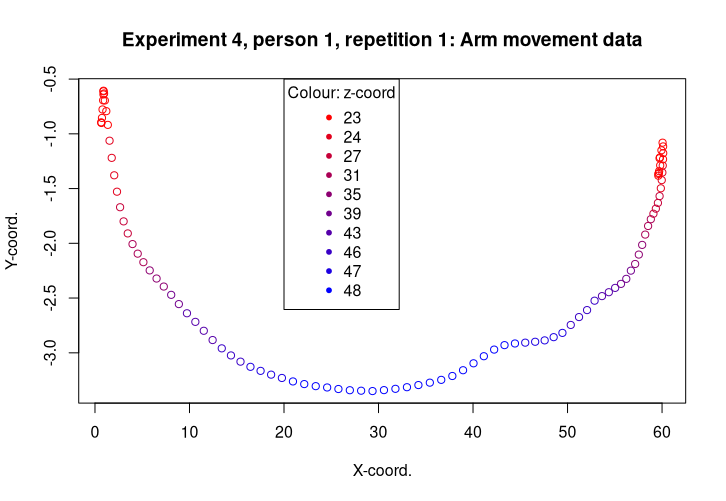
\includegraphics[width=.5\linewidth]{p1_example}
	}
	\subfloat{
		\centering
		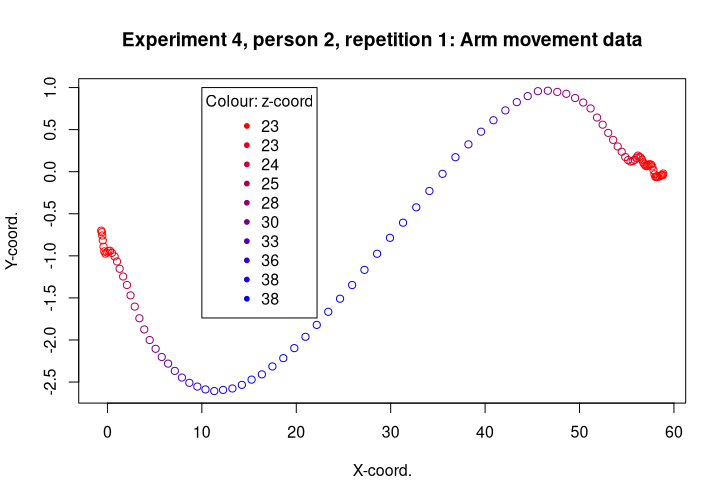
\includegraphics[width=.5\linewidth]{p1_example2}
	}
	\caption{Visualizations of the movement curves of the two first people. Especially in the \(y\)-coordinate, a difference in movement pattern can be seen.}
	\label{fig:2dtrajects}
\end{figure}\noindent 
For our purposes, it was beneficial to consider each recording of $ x, y, $ and $ z $ as a single feature, so we ravelled the data such that each repetition had $ 300 $ features with one observation each.
For the first part of the report, we investigated only experiment 4, so we had a total of 100 observations.
The target variable was the person who performed the movement, so the goal of our machine learning models was a 10-class classification.

Later, we tested wether or not the experiment had a significant effect.
For this, we ravelled the data points into a vector of length $ 480,000 $ and used different subsets, which is explained in more details in section \ref{subsec:expeffect}. 36 of the 480,00 data points were missing values set to NA and ignored in the analyses.

\begin{figure}[H]
	\centering
	\subfloat{
		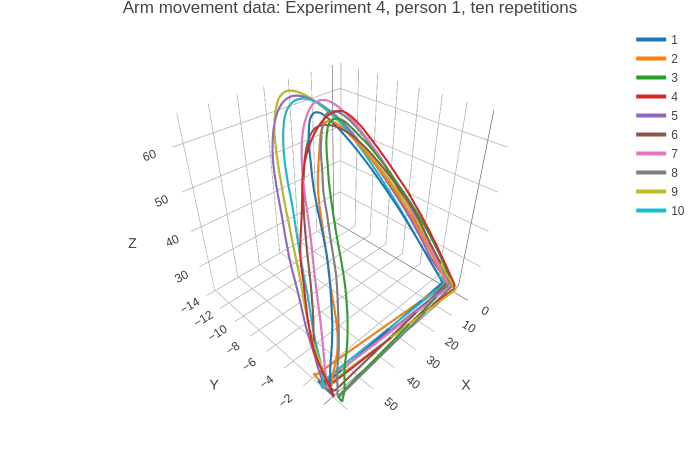
\includegraphics[width=.45\linewidth]{p1_3d_example1}
	}\hfill
	\subfloat{
		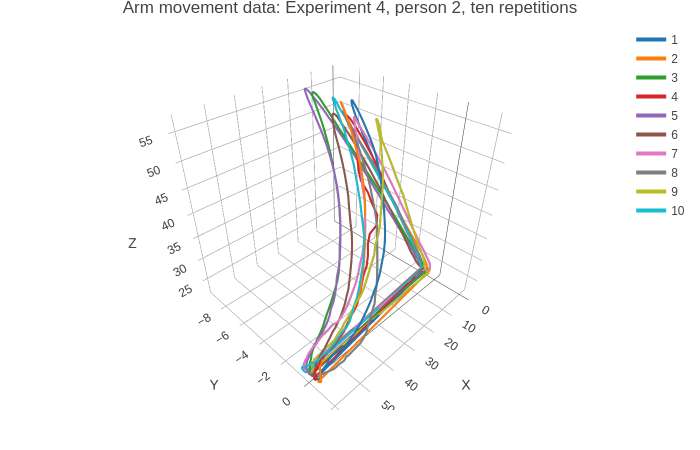
\includegraphics[width=.45\linewidth]{p1_3d_example2} 
	}
	\caption{Plots of some arm movements from experiment two.}
\end{figure}

\section{Methods and analysis}


\subsection{Machine Learning Task: Classification}
Two machine learning models were chosen to test on this 300-dimensional 10-class data.
It is noted from initial plots -- the title page figure and fig. \ref{fig:2dtrajects} -- that the effects of different people seem non-linear (at least the differences in their movement curves do), such that models that can model nonlinear decision boundaries are considered.
\paragraph{Models} The two chosen models were a binary classification tree and a 3-nearest neighbour classifier. The classification tree used the implementation of Hunt's algorithm of the \texttt{tree} package in \texttt{R} \cite{Tree}. For splitting criterion, the \textit{deviance} is used which is based on minus two times the log likelihood of the data under each model that the split results in \cite{Deviance}.

The second model was the \(K\)-nearest neighbour classifier which predicts classes using \(K\) nearest data points in the training set in euclidean distance and tie breaking by increasing \(K\) for the data point. This was implemented in the \texttt{R} package \texttt{class} \cite{KNN}. Before training on the data set, the hyper parameters of both models were defined and were not subject for testing. \(K\) was set to 3 as it was deemed suitable for the 10-class setting.

To evaluate the performance of the models, a classification baseline was set. As the classes are perfectly balanced, a baseline is expected to reach 10\pro\ accuracy. As no class is the largest, the baseline is constructed by randomly guessing classes to avoid skewing the evaluation towards any class as this might make a difference for the McNemar test.


\paragraph{Performance evaluation}
To evaluate which machine learning model best predicts the person completing the tasks, leave-one-out cross validation is implemented thus training the models on 99 data points and and testing on the last for each fold.
From here, 100 predictions are obtained which are used to achieve a point estimate for the accuracy of the classifiers.

To test whether the differences in the accuracy estimates are significant, McNemar's test is used. 
This test is used as described in \cite[Method 11.3.2]{Tue} and uses the beta distribution as a posterior to achieve a method for computing confidence interval of the difference in classifier accuracy.
From this test, a \(p\)-value for the null hypothesis that the two classifiers have the same accuracy can also be computed by using the binomial cumulative probability density function.

These tests consider the matched-pair matrix which counts the number of times the classifiers both are wrong, the number of times they both are right, the number of times one is better than the other (\(n_{12}\)) and vice versa (\(n_{21}\)).
Intuitively, this takes into account that some classifications might be more difficult than others. 
This is the motivation for the baseline consisting of random guesses.


\subsection{Test of experiment effect}\label{subsec:expeffect}
Analysis of Variance, ANOVA, is used to compare the mean positional values between the factors in the data with focus on detecting if there is a significant difference between the experiments.
This test of whether the overall mean is due to random variation using variability decomposition is done on a linear, two-way, multiplicative model:
\[
	y_{ij} = \alpha_{\text{experiment } i}+
	\beta_{\text{person } j}+ 
	\gamma_{\text{experiment } i \times\text{person } j }
	+ \epsilon_{ijkl}, \quad \epsilon_{ij} \sim \mathcal N (0, \sigma^2)
\]
The null hypothesis which was the focus of the test was $ H_0: \alpha_1=\alpha_2=\ldots=\alpha_{16} $ but the person was included to strengthen the test by taking the variance within this group into account and to fortify the assumption of independence. 
The interactions were included in the model to capture the entirety of the effects in the data and avoid the observations being non-independent.

Because ANOVA compares the means of different groups, it is relevant to compare the effect of the experiments one feature at a time.
We therefore ravelled all 480,000 data points in to a vector, and split them into subsets of $ 1,600 $ data points, each corresponding to one of the $ 300 $ coordinate features.
This also ensured independence between the observations, as e.g. an $ x_1 $ value would have had no influence on another.

Running ANOVA on resulted in the test containing 300 tests and thus returning 300 $ p $ values, each describing the effect of the experiment on a particular coordinate vector. These were then corrected with the Benjamini-Hochberg method \cite{BH}.


\section{Results}

\subsection{Classification models}

\paragraph{Point estimates for accuracy}

\begin{align*}
	& \hat \theta_{Base}= 12\pro 
	&& \hat \theta_{Tree} =41\pro 
	&&&\hat \theta_{3NN} = 60 \pro 
\end{align*}
\paragraph{Comparison of 3NN and classification tree}
Matched pair matrix:

\begin{table}[H]
	\centering
	\begin{tabular}{l|c c}
		&Tree is correct& Tree is wrong \\
		\hline
		3NN is correct &35& 25\\
		3NN is wrong& 6& 34
	\end{tabular}
\end{table}\noindent 
Estimate for accuracy difference, 99\pro\ confidence interval and \(p\)-value for \(H_0: \theta_{3NN}=\theta_{Tree}\):
\[
\widehat{\Delta \theta} = 19\pro,\quad  \Delta \theta\in[7\pro , 30\pro], \quad p = 0.0059 
\]

\paragraph{Comparison of 3NN and baseline}
Matched pair matrix:

\begin{table}[H]
	\centering
	\begin{tabular}{l|c c}
		&Baseline is correct& Baseline is wrong \\
		\hline
		3NN is correct &7& 53\\
		3NN is wrong& 5& 35
	\end{tabular}
\end{table}\noindent 
Estimate for accuracy difference, 99\pro\ confidence interval and \(p\)-value for \(H_0: \theta_{3NN}=\theta_{Base.}\):
\[
\widehat{\Delta \theta} = 48\pro,\quad  \Delta \theta\in[33\pro , 61\pro], \quad p = 3.5\ctp{-11}
\]

\paragraph{Comparison of classification tree and baseline}
Matched pair matrix:

\begin{table}[H]
	\centering
	\begin{tabular}{l|c c}
		&Baseline is correct& Baseline is wrong \\
		\hline
		Tree is correct &2& 39\\
		Tree is wrong& 10& 49
	\end{tabular}
\end{table}\noindent 
Estimate for accuracy difference, 99\pro\ confidence interval and \(p\)-value for \(H_0: \theta_{Tree}=\theta_{Base.}\):
\[
\widehat{\Delta \theta} = 29\pro,\quad  \Delta \theta\in[14\pro , 43\pro], \quad p = 3.8\ctp{-5}
\]

\subsection{Impact of experiment}
The results of the 300 two-way ANOVA's is given below. With \(N\) sign. tests is meant the amount of tests significant at \(\alpha = 0.01\). BH is referring to the Benjamini-Hochberg adjustment to account for the 300 tests. The \(\overline{ MSE}\) is computed as the average of the 300 MSE's.
\begin{table}[H]
	\centering
	\begin{tabular}{l | c c c c}
		300 ANOVA's & \(\overline{MSE}\) & \(N\) sign. tests& \(N\) BH-sign. tests& Freq. BH-sign. tests\\
		\hline 
		Experiment  & 659 	& 258 & 258 	& 86\pro	\\
		Person  & 648 		&  300 & 300	&100\pro  \\
		Experiment\(\times\)Person&7.61  & 218 & 217 &	72\pro	\\
		Residuals &3.6 &			
	\end{tabular}
	\label{tab:ranova}
\end{table}\noindent
The distribution of \(p\)-values of the experiment can be seen below in figure \ref{fig:sortp}.
\begin{figure}[H]
	\centering
	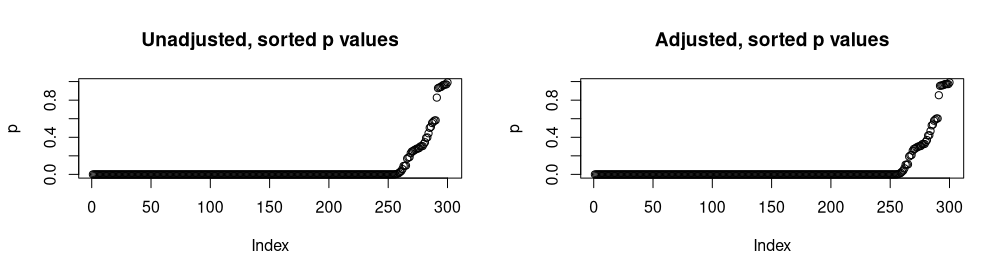
\includegraphics[width=.8\textwidth]{pvalues}
	\caption{Sorted $ p $ values. On the right figure, they are adjusted using the Benjamini-Hochberg correction algorithm.}\label{fig:sortp}
\end{figure}

\section{Discussion and Conclusion}
\paragraph{Validity of statistical analyses}
The parametric McNemar test is noted to be an approximation from asymptotic theory and the source \cite{Tue} states that the \(p\) values and confidence intervals should be considered together and that they only hold when \(n_{12}+n_{21}> 5\). This is seen to hold for all the matrices (the sums being 31, 58 and 49 for the comparisons) such that the results of the McNemar comparisons are seen as accurate.
\begin{figure}[H]
	\centering
	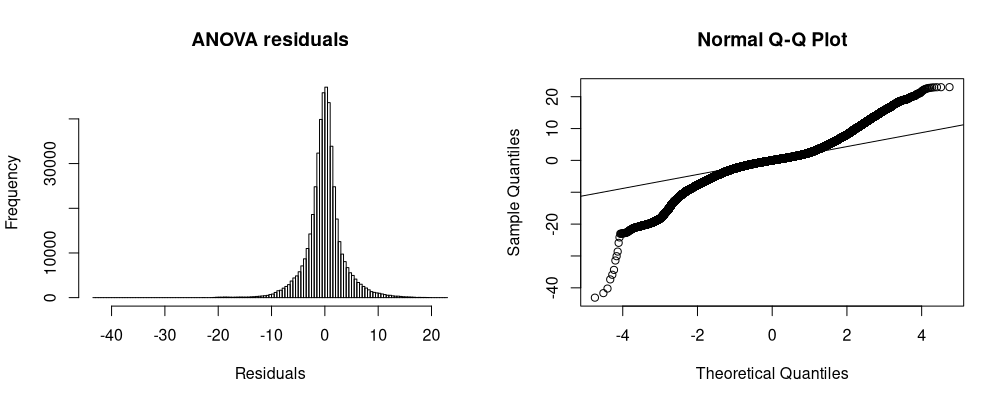
\includegraphics[width=.9\textwidth]{qq}
	\caption{Quantile/quantile-plots of the residuals of twelve of the 300 ANOVA models. Major problems are only seen in the bottom rightmost.}\label{fig:qq}
\end{figure}\noindent
For the 300 two-way ANOVA's, it is challenging to visualize the important assumptions of residual normality and residual variance homogeneity. An arbitrary subset of the 300 tests is thus chosen and visualized. Figure \ref{fig:qq} substantiates the assumption of normality as only minor outliers and non-normal tendencies can be seen. These residual populations are also visualized as histograms in the appendix, figure \ref{fig:residuals}.

The assumption of variance homogeneity for the \textit{experiment} factors is in the same vein visualized by boxplots of these same 12 coordinate features. 
From this (somewhat overwhelming) plot at figure \ref{fig:vars}, the assumptions seem reasonably well fulfilled at the given zoom level as only few of these coordinate tests have experiment levels with visibly differing variance.  
The assumption of independence of the errors is regarded as fulfilled between the groups of experiments and people, but the repetition number was not included in the ANOVA such that this could be a source of unmodelled grouping of the data though it should not be a significant factor in a well designed experiment. 


For this large amount of tests, the assumptions in each are not fully tested. 
Thus, to achieve precise measurements of number of significant tests, the model validation should include  full investigation of residual distribution including search for nonlinear effects in the tests.
Furthermore, examinations of variance homogeneity with regards to the \textit{person} factors and the interactions should be carried out. 
%The four-way ANOVA on the other hand has some major issues with model assumptions. The assumption of independence is arguably realized as all observations are fully divided by these four groups. This was also the motivation for doing the full four-way analysis and including each single of the 300 coordinates as a factor. It must, however, be noted that interactions between these four groupings were not tested.
%
%The assumption of residual variance homogeneity is visualized with boxplots. For \textit{experiment}, which is the goal of this test, it seems reasonable bar some outliers, especially in experiment 5, at this zoom level. Similar boxplots for person and repetition are included in the appendix  at figure \ref{fig:vars} and look very similar with single outliers.
%\begin{figure}[H]
%	\centering
%	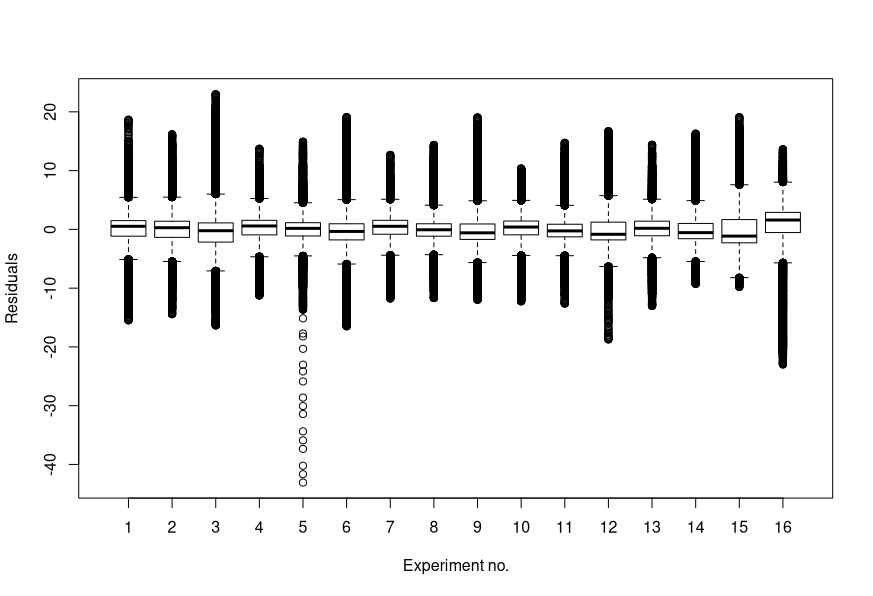
\includegraphics[width=.7\textwidth]{var_exp}
%\label{fig:vexp}
%\end{figure}\noindent
%Finally, the assumption of residual normality of ANOVA is checked using a histogram and a quantile/quantile visualization. This assumption shows clear problems: The residual distribution is too narrow for the normal bell curve and has long tails and negative outliers. This severely limits the accuracy of the statistical claims of the ANOVA and results in a higher risk of type I errors than the \(p\) values indicate.
%\begin{figure}[H]
%	\centering
%	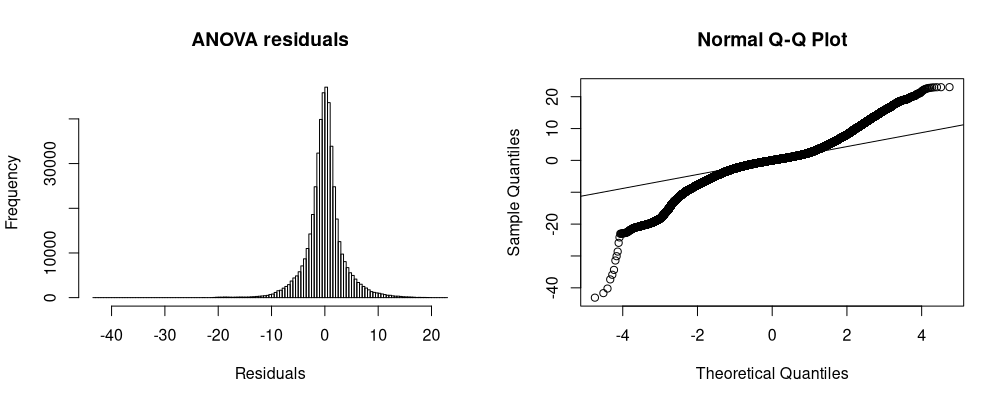
\includegraphics[width=.7\textwidth]{qq}
%	\caption{Histogram and quantile/quantile-plot of the residuals of the ANOVA model.}\label{fig:qq}
%\end{figure}

\subsection{Classification of persons}
%The initial visualizations of the data in the 3D and 2D scatter plots -- \ref{fig:trajects} and \ref{fig:2dtrajects} -- showed clear differences between the repetitions of the first two people that humans would be able to classify visually especially it is seen that there is a clear difference in the way these two people move in the \(y\)-direction.  
It is seen that the expectation of some accuracy on the person classification task was confirmed: The 3-nearest neighbour model is the best at 60\pro\ and is significantly better than the classification tree and they are both significantly better than the random guesses. The greater aim of reliably discerning people based on movement is far from achieved at an performance of 60\pro. However, this significant result with these un-optimized models shows a promise for the machine learning task as there is a number of possible improvements. 



The models were not tested for complexity controlling hyper parameters such as \(K\) for the KNN or the impurity function for the tree model and possible improvements could be found here. A larger improvement could be found in much more complex models for this high-dimensional data set such as random forests or deep neural networks. More generalizable performance could also be found by using the entire data set, not just experiment 4, to find more general personal  features and mannerisms.

\subsection{Test of difference in experiments}
As no data is a perfect representation of reality, under the null hypothesis, it would still be expected to find that $ 1\pro $ of the non adjusted $ p $ values are significant at a $ 1\pro $ significance level. However, we found that, even after correcting the $ p $ values, 86\pro\ of them were significant at our significance level of $ 1\pro $.
\begin{figure}[H]
	\centering
	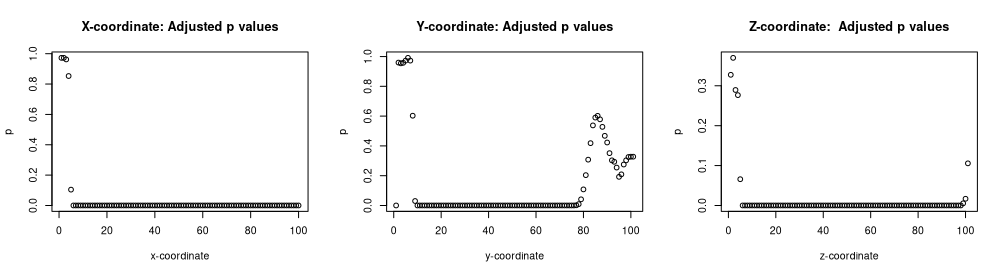
\includegraphics[width=.8\textwidth]{coordinate_ps}
	\caption{Benjamini-Hochberg corrected $ p $ from the 300 ANOVA \(F\) tests divided based on their corresponding coordinate features.}\label{fig:unsortp}
\end{figure}\noindent 
It is noted with some surprise that the \(p\)-value adjustments had very little effect. This is connected to the high-variance \(p\)-value distribution which shows that most values are very close to 0 but a minority have dramatically higher \(p\)-values as can be seen in figures \ref{fig:sortp}, \ref{fig:unsortp}. To understand this distribution, figure \ref{fig:unsortp} shows the \(p\)-values sorted after the test's corresponding coordinate.  
A common sense expectation could explain this: The high \(p\)-values -- where the means of the experiments are very similar -- occur at the beginning and end of the coordinates as most experiments start and end in the same way. 
Especially the \(y\) coordinate shows high \(p\) values in the end suggesting that the experiments are designed in a way where similar movements are needed in the \(y\)-direction in the end. 
This sharp division of the tests is further amplified by numeric underflow as 19\pro\ of the \(p\)-values are below floating point precision and are coerced to 0.
\\\\
As the goal of the tests was to find if it was possible to distinguish the experiments from these tests, the null hypothesis can be rejected as this overwhelming amount of significant tests gives a high degree of evidence against the experiment being without effect on the curves.
This conclusion is seen as significant even though some normality and independence assumptions are not fully tested as such convincing amount of evidence is found.
 
The test method could be improved by performing non-parametric tests which do not require normality, using feature-specific data transformations to help improve the normality of the residuals or including the repetition factor.

The experiment also had an effect in connection  with the person as the tests found significant effects of the interaction between these at \(72\pro\) of the tests though this on average explained much less of the variability than the other groups.

The \textit{person} factor was found to have significant differences on every one of the 300 tests. Person-to-person variability in arm movement is thus so high that differences between these 10 people can be found in every coordinate -- a result which gives further credence to the possibility of success in the human movement classification task.






%The ANOVA finds that the experiment had a statistically significant impact on the hand movements of the test subjects with $ p<2.2\ctp{-16} $.
%This was also the case for every individual experiment which was found to be different from the control with the smallest estimeate mean difference being experiment 3 with \(0.252\) and the largest being experiment 14 with \(3.22\).
%There was also, as could be expected from partial success of the machine learning task, found differences in the person. Even the repetition was found to be significant although it explains the least amount of variability of all the groupings at \(MSE_{repetition}=1,115\) while experiment explains \(MSE_{experiment}=28,910\).
%
%However, the normality assumption of the ANOVA test utilized was not realized which means that the very low \(p\) values cannot be taken as the actual risk of type I errors. 
%Nevertheless, \textit{experiment} was the grouping that explained the next to highest amount of  variability after the obviously important \textit{coordinate} factor. 
%This fact, together with the fact that the ANOVA comparatively had such a low residual error at \(MSE_{res.}=13\) and the amount of data points add up to a reasonable amount of evidence for the fact that the experiments have significant effects on the movement curves. 
%
%To test this conclusion further, non-parametric rank-sum tests or bootstrapping to achieve normality should be implemented.


\newpage
\begin{thebibliography}{9}
	\bibitem{BH} Benjamini, Y and Hochberg, Y: "Controlling the False Discovery Rate: A Practical and Powerful Approach to Multiple Testing", 1995.
	\bibitem{Tue} Herlau, T et al. "Introduction to Machine Learning and Data Mining: Lecture notes, Fall 2019, version 1.4b" 13/12-19.
		\bibitem{kine} The University of British Columbia: School of Kinesiology:
	"Neuromechanical Studies in Kinesiology". \\
	At:
	\url{https://kin.educ.ubc.ca/research/neuro-mechanical/} (consulted 19/01-20)
	\bibitem{KNN} Ripley, B.: "Package ’class’", 01/01-19 .\\
	At:
	\url{https://cran.r-project.org/web/packages/class/class.pdf} (consulted 16/01-20)
	\bibitem{Tree} Ripley, B.: "Package ‘tree’", 26/05-19.\\ At: \url{https://cran.r-project.org/web/packages/tree/tree.pdf} (consulted 16/01-20)
	\bibitem{Deviance} Ritschard, G.: "Computing and using the deviance with classification trees", 01-06.\\
	 At:
	\url{http://mephisto.unige.ch/pub/publications/gr/ritschard_compstat06.pdf} (consulted 16/01-20)
	\url{http://www.math.tau.ac.il/~ybenja/MyPapers/benjamini_hochberg1995.pdf} (consulted 20/01-20)

\end{thebibliography}
\appendix
\newpage 
\section{Figures}

\begin{figure}[H]
	\centering
	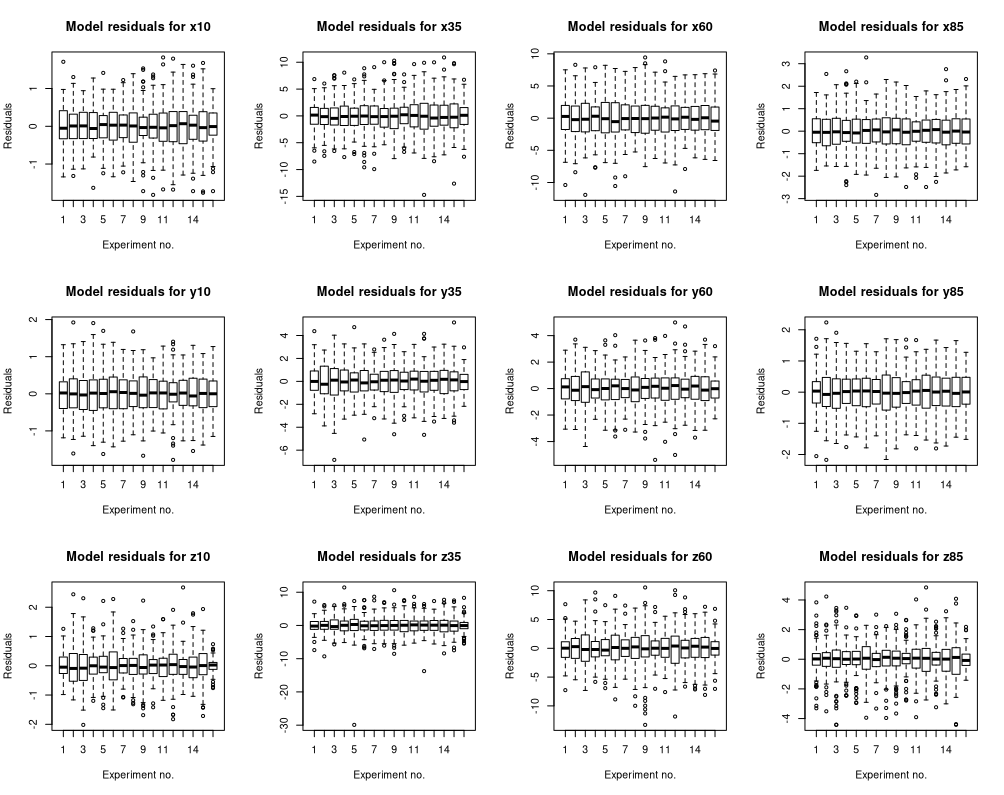
\includegraphics[width=\linewidth]{var_experio}
	\caption{Visualization of the residual distributions of some of the coordinate features. }
	\label{fig:vars}
\end{figure}



\begin{figure}[H]
	\centering
	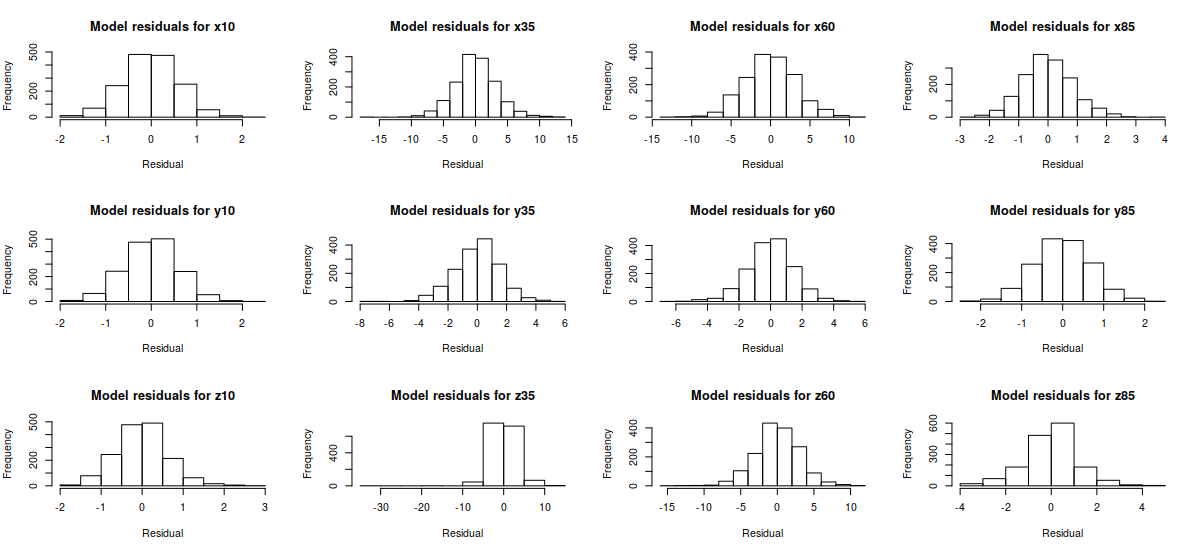
\includegraphics[width=\textwidth]{residuals}
	\caption{Distributions of the residuals of linear models for some of the coordinate features.}\label{fig:residuals}
\end{figure}

\end{document}

















